\begin{figure}
    \centering
    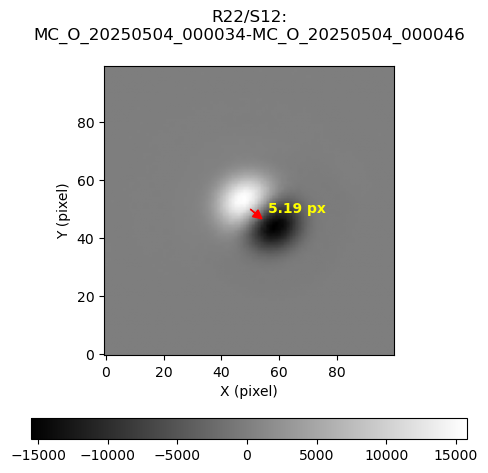
\includegraphics[width=0.45\linewidth]{onskyperformance/filterplacement/diffimage.png}
    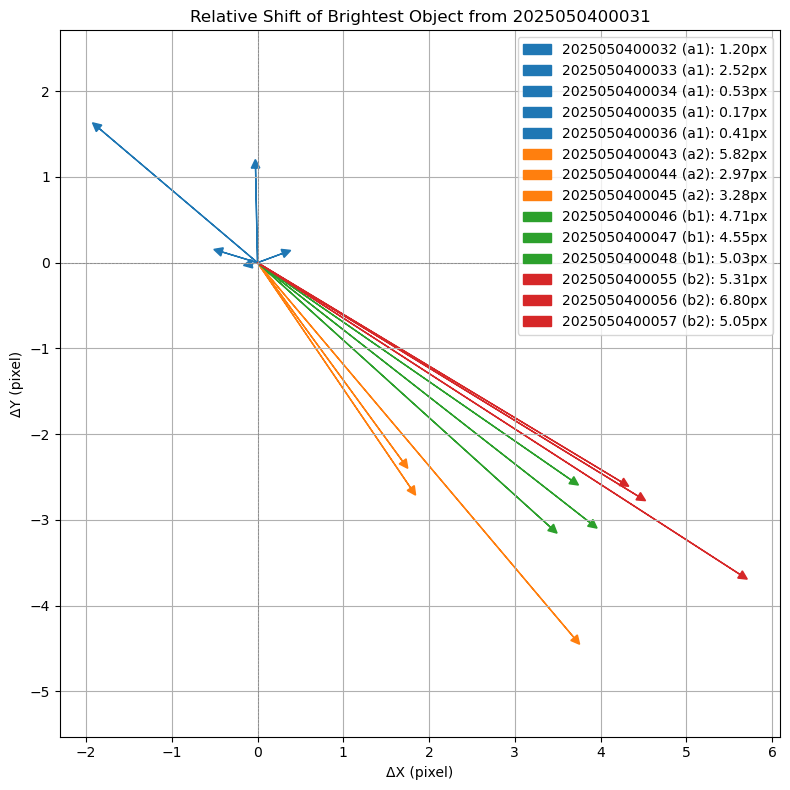
\includegraphics[width=0.45\linewidth]{onskyperformance/filterplacement/total.png}
    \caption{Caption}
    \label{fig:placeholder}
\end{figure}
During the commissioning campaign we used the Collimated Beam Projector (CBP) to project a spot through the pinhole filter onto the LSSTCam focal plane. The main focus was on the repeatability of the filter placement by comparing the position of the spot before and after swapping the filter.

The image acquisition was carried out in a systematic sequence that combined three LSSTCam rotator angles (0\degree, 18\degree, and -72\degree) with two CBP mask sizes (5\,mm and 3\,mm). For each combination we obtained several exposures before the filter swap and one after, yielding a total of 51 images. The exposures were taken in the order shown in Table \ref{tab:acquisition}; the exposure that was marked “IGNORE” was omitted from the analysis. 
\begin{table}[h!]
\centering
\begin{tabular}{cccc}
seqNum & Rotator angle (deg) & CBP mask (mm) & Before/After swap \\
\hline
31–36  & 0   & 5 & Before \\
37–40  & 18  & 5 & Before \\
41–44  & –72 & 5 & Before \\
45–50  & 0   & 5 & After \\
51–56  & 18  & 5 & After \\
57–62  & –72 & 5 & After \\
63–68  & 0   & 3 & Before \\
69–74  & 18  & 3 & Before \\
75–80  & –72 & 3 & Before \\
81–86  & 0   & 3 & After \\
87–92  & 18  & 3 & After \\
93–98  & –72 & 3 & After \\
\end{tabular}
\caption{Sequence of exposures used for the filter-placement test. The table shows, for each exposure, the rotator angle, CBP mask diameter, and whether the exposures were taken before or after the filter change.}
\label{tab:acquisition}
\end{table}


The left-hand panel of Figure~\ref{fig:placeholder} shows a difference image between the first exposure before the filter change and the fourth exposure after the filter change, revealing small but systematic shifts in the pinhole positions. The right-hand panel displays the measured positional offsets relative to the first exposure for images that are taken when the rotator angle was 0\degree. Scatter within a single condition (e.g., all points from a1) is on the order of a few pixels, indicating that the CBP itself is stable but non-negligible motion could be present. 

Systematic offsets are evident when comparing conditions: the average shift between a1 and b1 is $\approx$ 2 px in X and $\approx$ 3--4 px in Y. The four distinct groups (a1, a2, b1, b2) are distributed reasonably consistent but distinguishable distributions. Because the total displacements are well below the 10-pixel (100 µm) repeatability requirement, we conclude that the filter placement is within specification. Nevertheless, the observed systematic trends suggest that both filter positioning and rotator repeatability contribute to the measured offsets, making it difficult to isolate the dominant source without further controlled experiments.


